Here we model the systematic errors on the stacked cluster weak
lensing measurement by comparing the average mass in each bin
to the mass measured by a shear profile, affected by shape 
measurement bias. To measure the effect of shape measurement bias, a \citet*{1997ApJ...490..493N} (NFW) density profile is created for each mass bin. This density profile is
used to calculate the tangential reduced shear $g$ as described in \cite{NFW}. \\

\iffalse
\green{I don't think we need this}
\indent The NFW density profile is given by
\begin{equation}
\rho(r) = \frac{\delta_c\rho_c}{(r/r_s)(1+ r/r_s)^{2}}
\end{equation}
where $\rho_c = \frac{3 H^2 (z) }{8 \pi G} $ is the critical density , $
H(z) $ is Hubble's parameter , $G$ is Newton's constant, $r_s =
r_{200}/c$, $c$ is the concentration and 
\begin{equation}
\delta_c = \frac{200}{3}\frac{c^3}{ln(1+c) - c/(1+c)}
\end{equation}
from \citep{NFW} . The reduced shear from a NFW
halo is 
\begin{equation}
g = \frac{\gamma}{1-\kappa} = \frac{ \Delta \Sigma / \Sigma_c }{1
-\overline{\Sigma}/ \Sigma_c}
\end{equation}
\fi

The reduced shear as measured including shape bias is modeled as 
\begin{equation}
g' = (1+m)g + qg^2 \; .
\end{equation}
We then fit this $ g' $ distribution to get a $M_{200}$ and $ c $
value. \green{need more details here ... I guess sources uniformly distributed in area over some range in radius, maximum likelihood?}

\green{interpretation of results; note that even if the systematic offset is within the statistical uncertainties in each bin, all bins combinedly being measured low is a different story... at least need to discuss that}

\begin{figure*}
 \centering  % this centres figure in column
  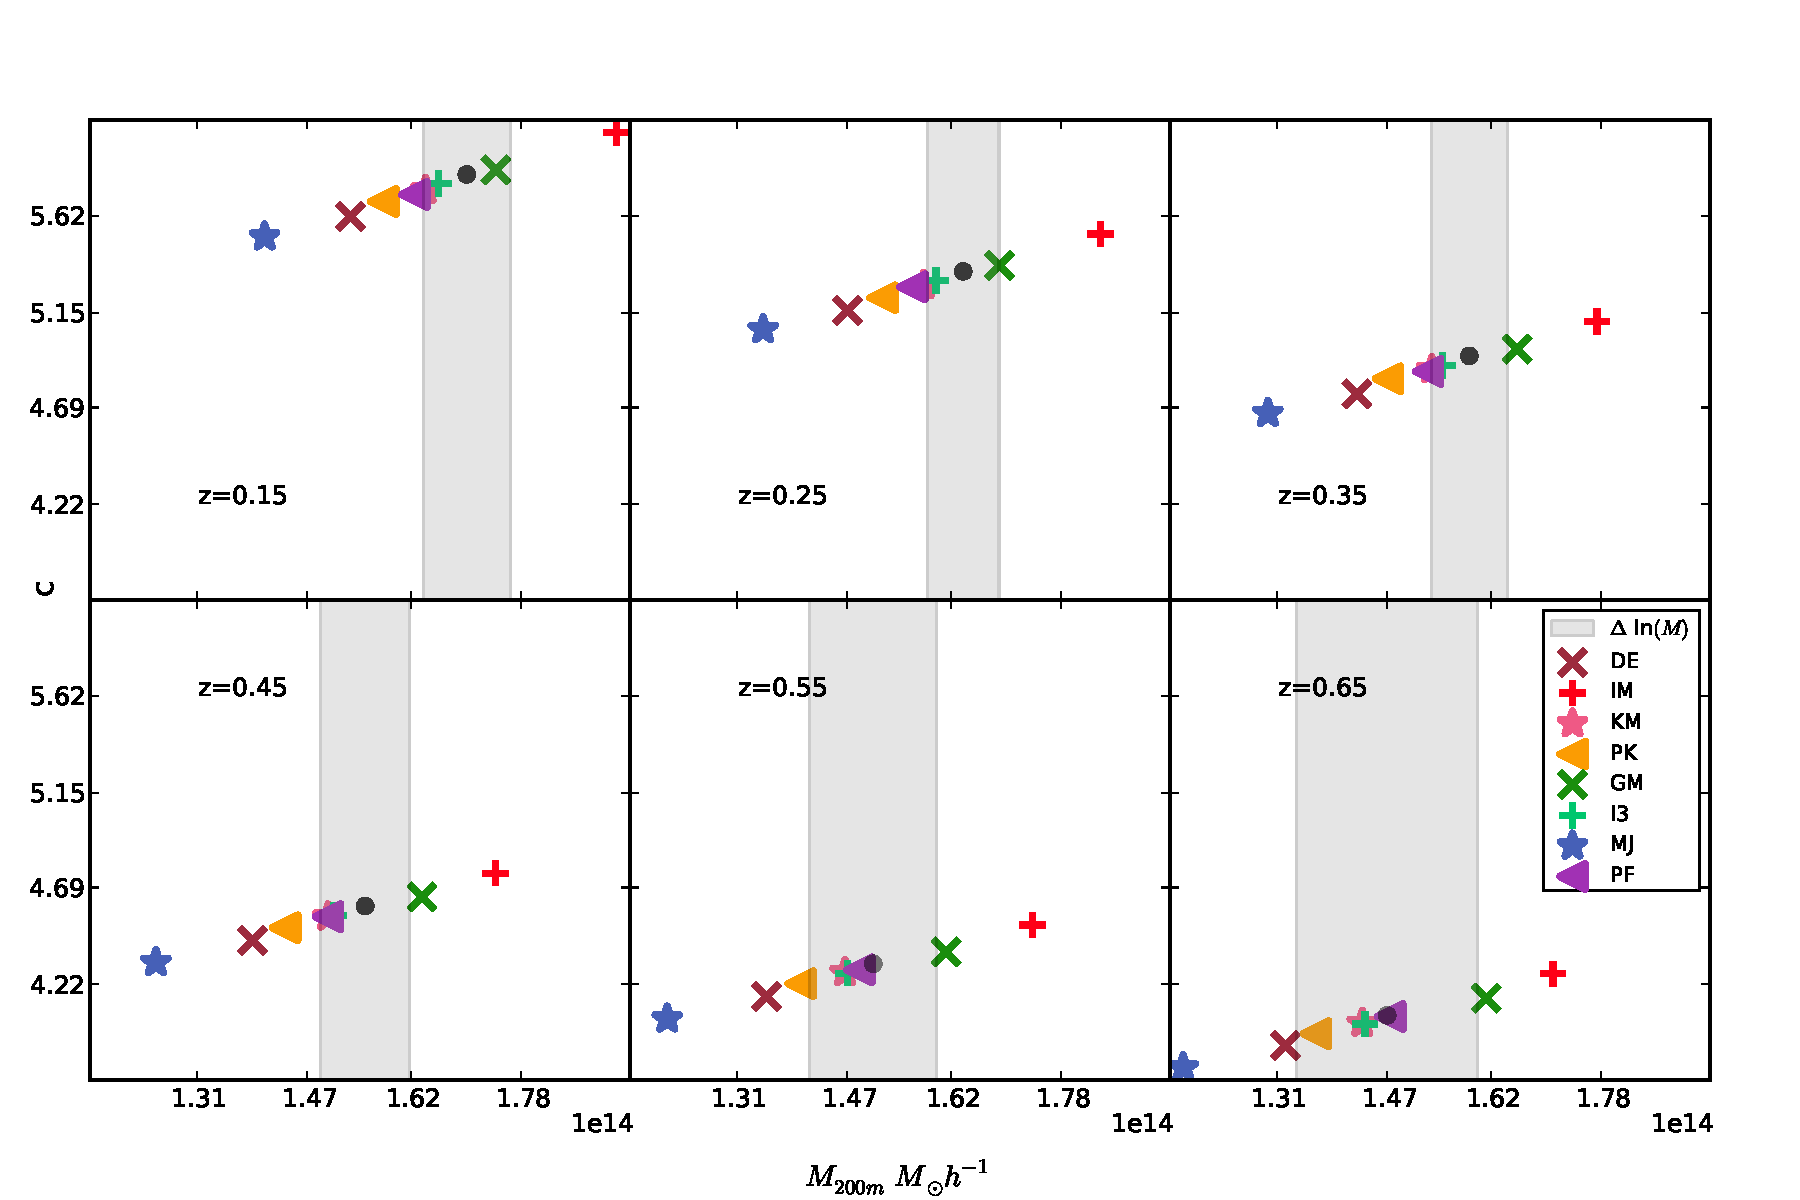
\includegraphics[width=0.95\textwidth]{fig/M_NFW_1.pdf} 
  \caption{NFW mass and concentration measured on a reduced shear
    profile affected by shape measurement bias
   as measured on all images for galaxy objects with SNR $>$ 20.}
\label{fig:M_NFW_1}
\end{figure*}

\begin{table*}
        \centering
        \begin{tabular}{|c|c|c|c|c|c|}  
          \hline
          N  &  $Z_{lens}$ & $Z_{source}$  & C & $M_{200m}$ $ M_\odot
          h^{-1}$  & $\Delta$ ln$(M)$ \\ 
          \hline
          450  & 0.16  & 0.58  & 5.82  & 1.70  & 0.037   \\
          \hline
          1080  & 0.26  & 0.62  & 5.35  & 1.64  & 0.032   \\
          \hline
          1744  & 0.35  & 0.66  & 4.94  & 1.59  & 0.035 \\
          \hline   
          2396  & 0.45  & 0.73  & 4.60  & 1.55  & 0.042   \\
          \hline
          2753  & 0.55  & 0.79  & 4.32  & 1.51  & 0.061   \\
          \hline
          3054  & 0.65  & 0.87  & 4.07  & 1.47  & 0.089   \\         
          \hline
        \end{tabular}
        \caption{ The expected statistical error due to one method of
          cluster stacking for a DES-like cluster distribution).}
    \label{table:NFW_1_b}
\end{table*}
